% inkscape sierpinski-square-curve.pdf --export-type=png --export-filename=sierpinski-square-curve.png --export-width=1024 --export-background-opacity=0
% \documentclass[a3paper]{article}
% \usepackage[left=0mm,top=1cm,right=0mm,bottom=0mm]{geometry}
\documentclass[border=0]{standalone}
% \documentclass[dvisvgm]{minimal}
\usepackage{tikz}
\usetikzlibrary{calc,lindenmayersystems}
\usepackage{xcolor}
\definecolor{pGreen}{HTML}{663366}
\pgfdeclarelindenmayersystem{Sierpinski Square Curve}{
\symbol{X}{\pgflsystemdrawforward}
\symbol{F}{\pgflsystemdrawforward}
\symbol{+}{\pgflsystemturnright} % Explicitly define + and - symbols.
\symbol{-}{\pgflsystemturnleft}
\rule{X -> XF-F+F-XF+F+XF-F+F-X}
}
\begin{document}
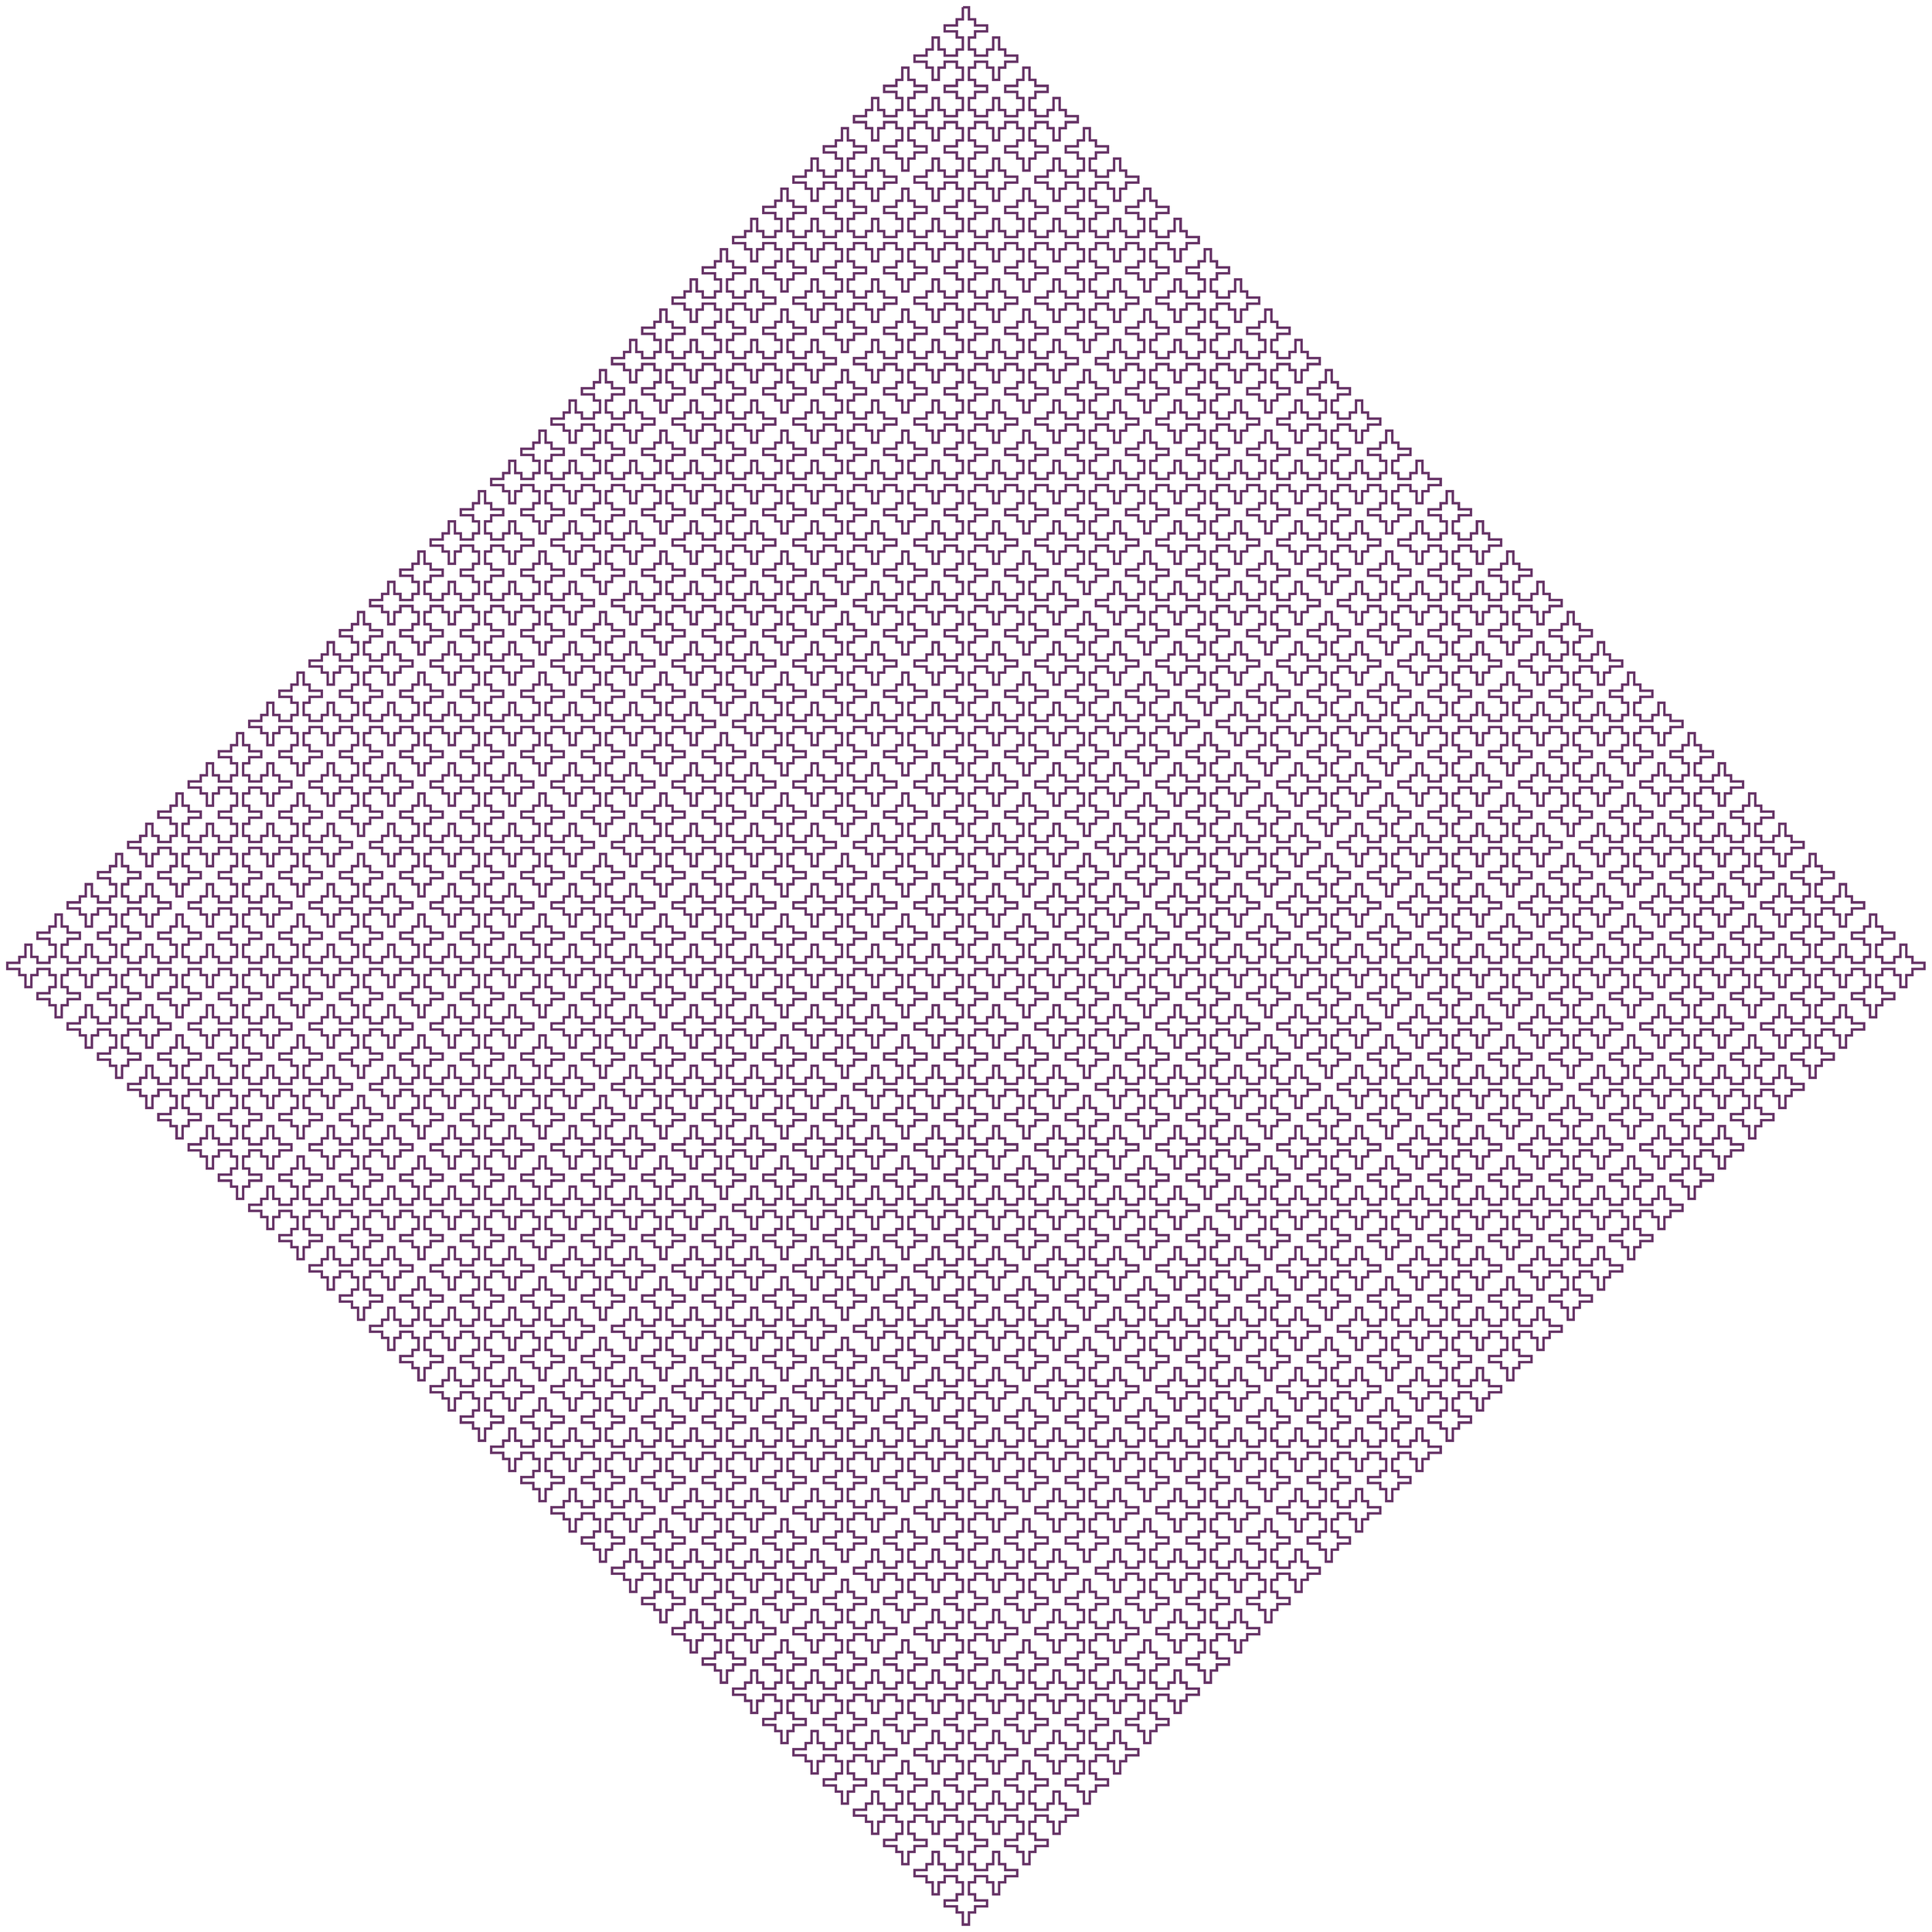
\begin{tikzpicture}
      \draw[lindenmayer system={Sierpinski Square Curve, step=10, axiom=F+XF+F+XF, order=6, angle=90},pGreen,line width=4pt] lindenmayer system;
\end{tikzpicture}
\end{document}